\section{Quantum Addition}
\label{sec:addition}

Updating the occupancy of a bosonic mode when applying bosonic ladder operators requires adding a classical number ($+ R - S$) to the register storing the occupation of the bosonic mode.
Controlled (modular) addition of a two quantum registers (storing the numbers in binary) can be performed using $2N - 3$ left (and right) elbows and $M - 1$ ancillae using the construction for addition introduced in \cite{gidney2018halving} (Figure 4):
\begin{equation}
    (\alpha \ket{0} + \beta \ket{1})\ket{m}\ket{n} \rightarrow \alpha \ket{0}\ket{m}\ket{n} + \beta \ket{1}\ket{m}\ket{n \oplus m}
\end{equation}
where $m$ is the value being added to $n$ and $M$ and $N$ are the lengths of the registers respectively.

When performing a bosonic occupancy update, the value of $m$ is a known, \textit{classical} value ($+ R - S$).
Naively, this could be performed by loading the value of $m$ into a clean register and then performing controlled addition of the two registers as described above.
However, since the value of $m$ is classial and known, there are a few other options.

\begin{figure}
    \centering
    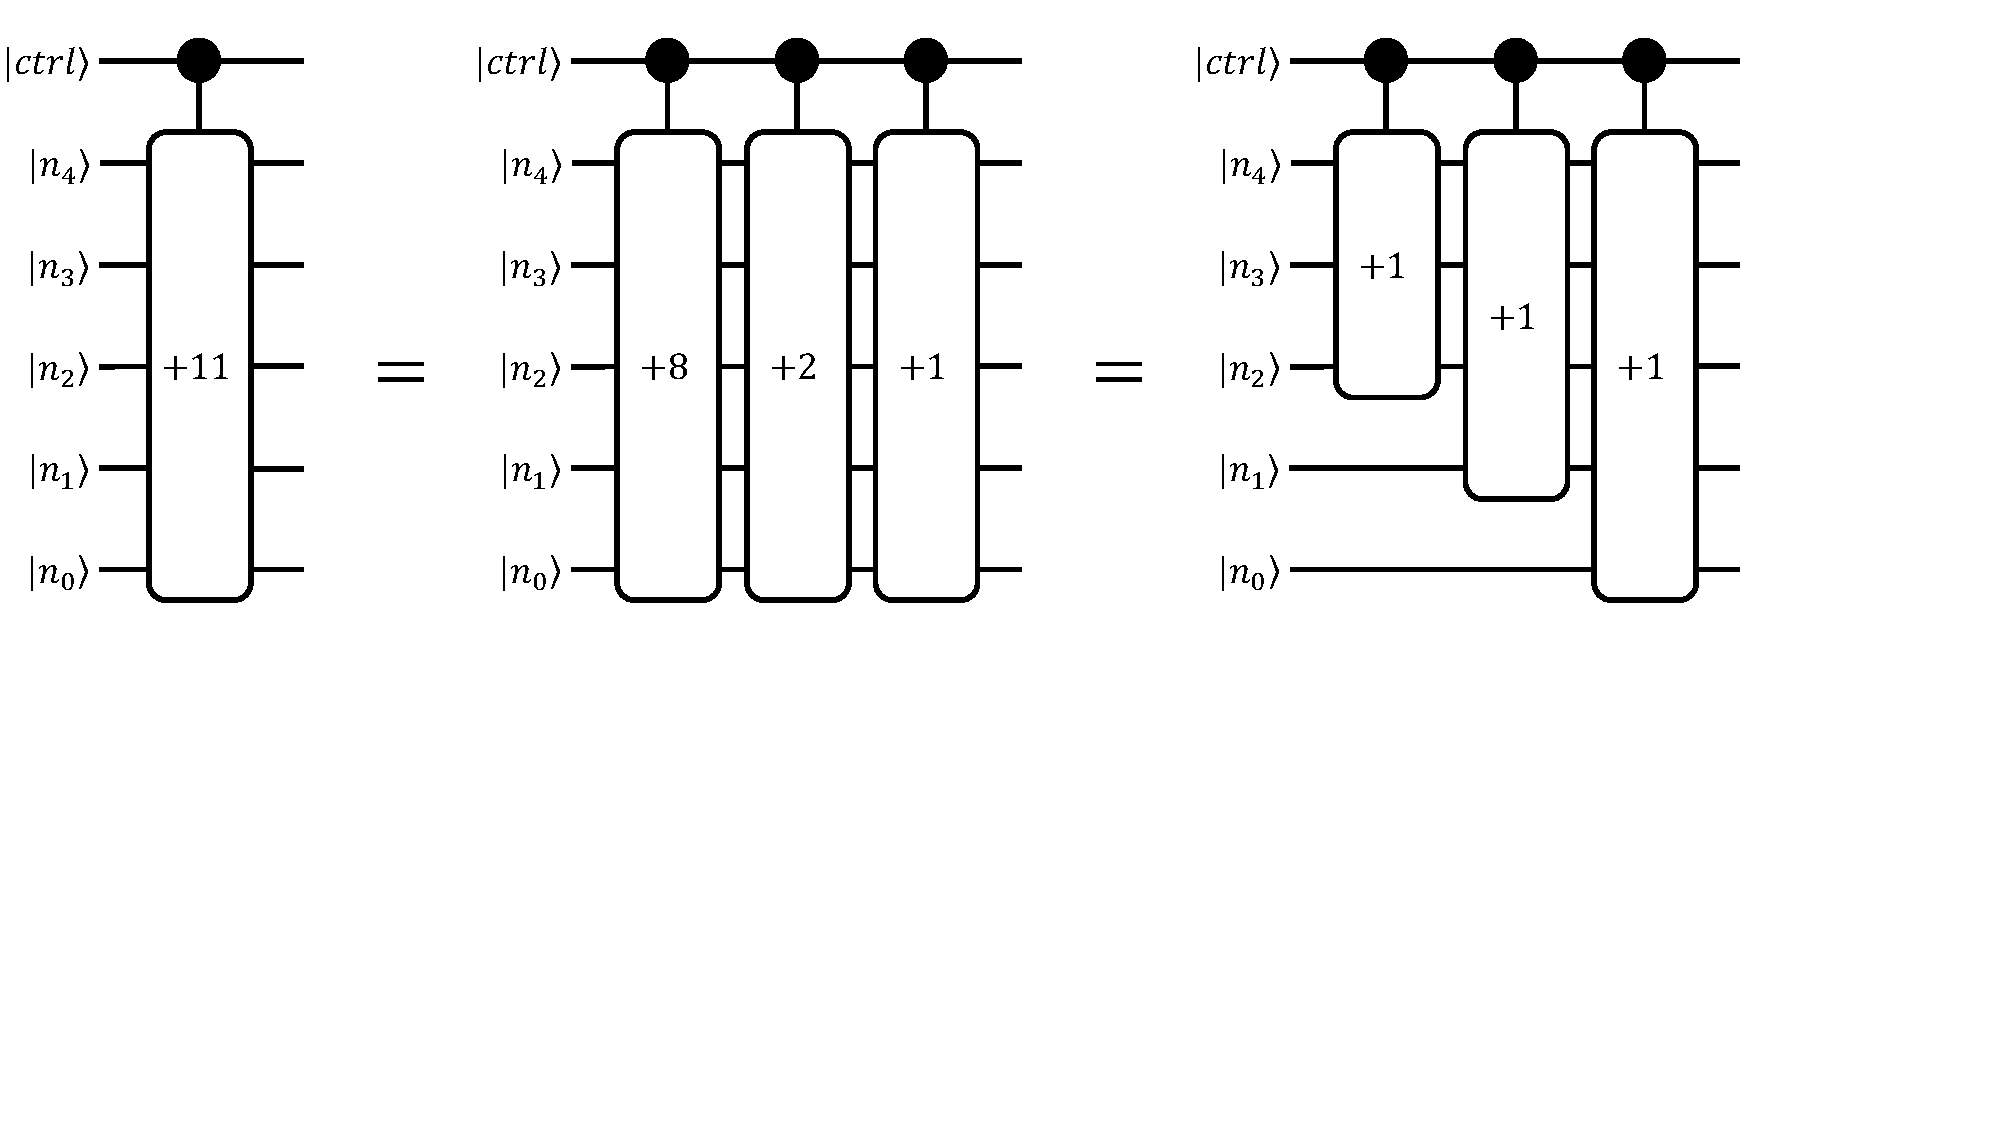
\includegraphics[width=16cm]{figures/addition-via-incrementers.pdf}
    \caption{
        \textbf{Addition via Incrementers} 
        This figure depicts an implementation of addition (mod $32$)by a classical value using a series of incrementers.
        An incrementer applied onto a register, excluding the least-significant qubit, implements a bit-shifted incrementer, leading to addition by $2$. 
        Addition by the classical value $11$ can be constructed by bit-shifted incrementers of $+8$, $+2$, and $+1$.
        Subtraction by the same value can be achieved by applying Pauli-X gates on each qubit before and after the operation.
    }
    \label{fig:addition-via-incrementers}
\end{figure}

\begin{figure}
    \centering
    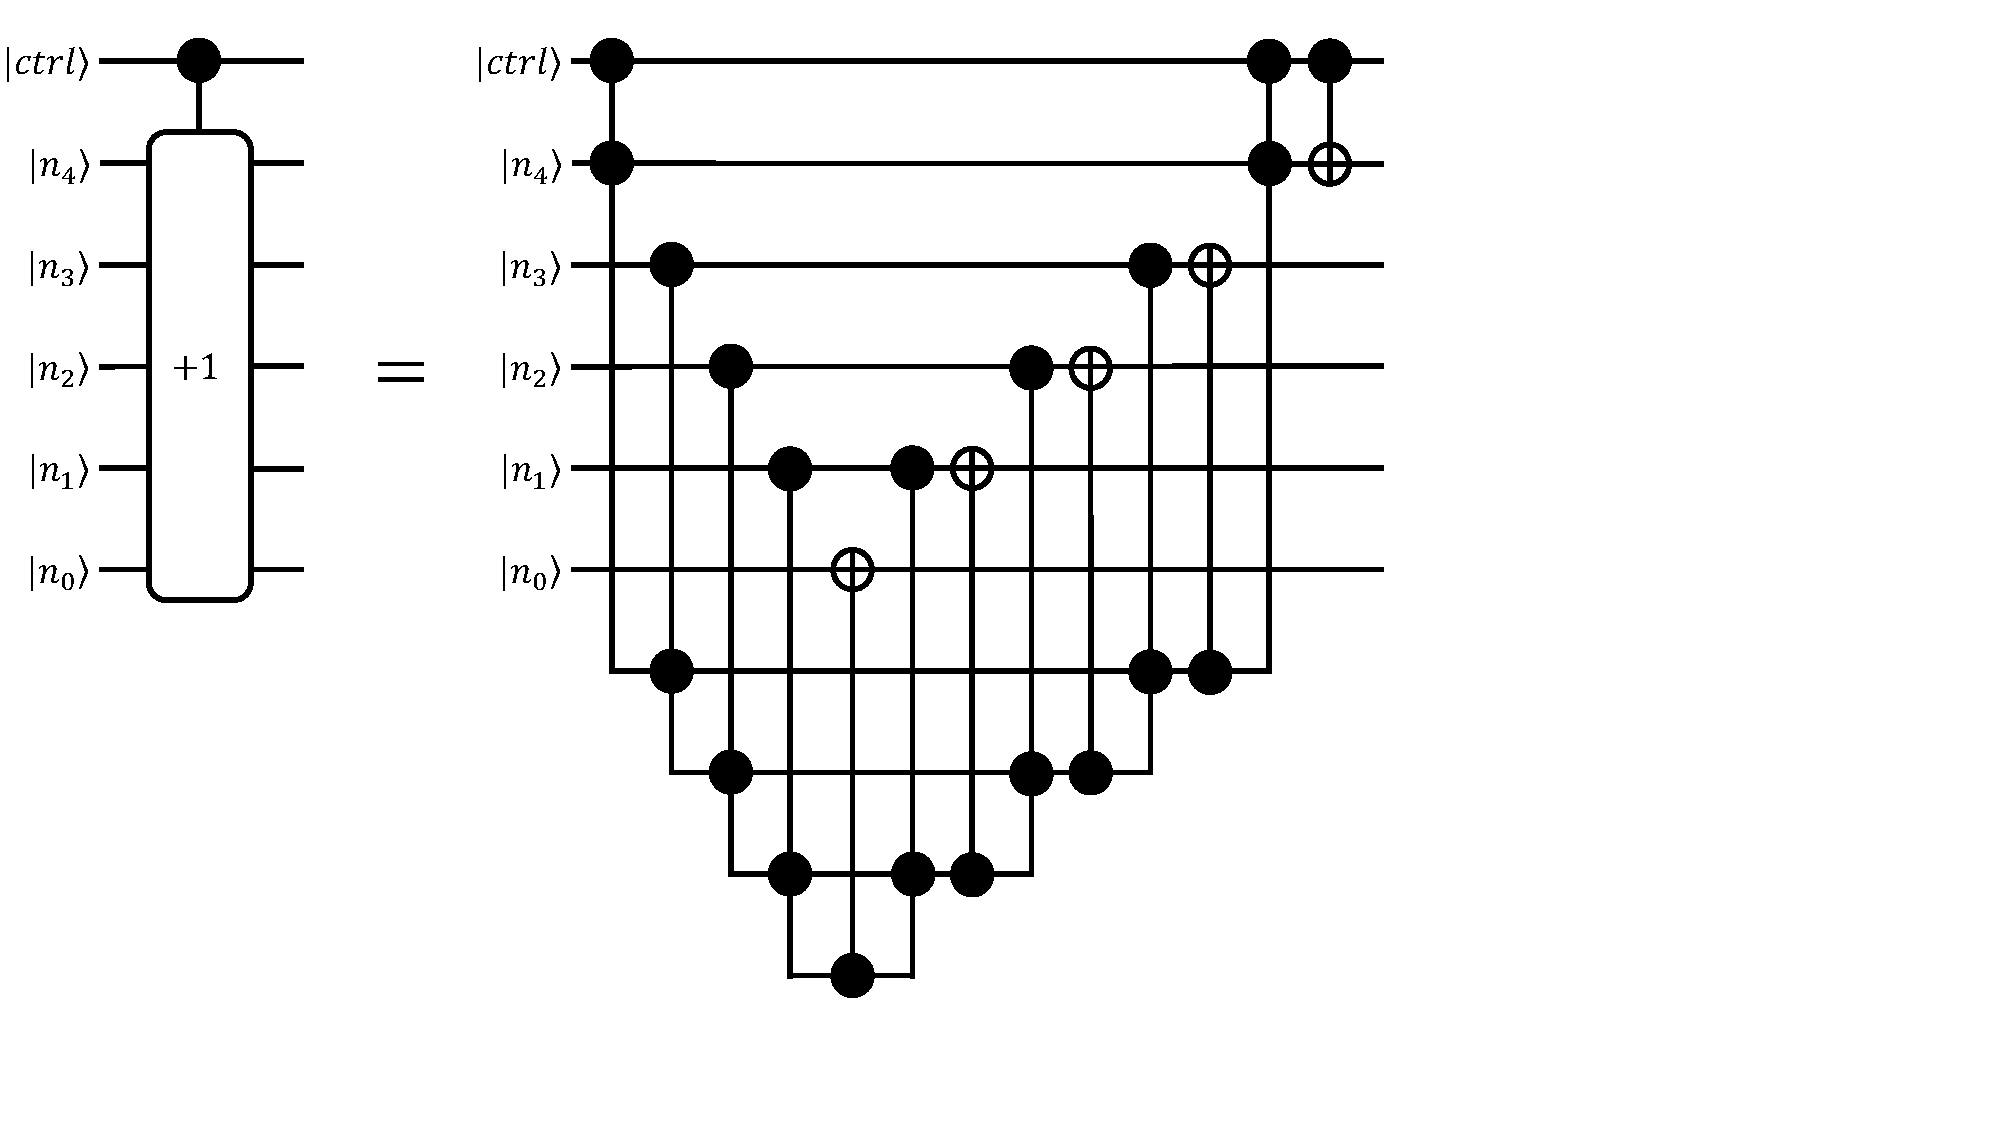
\includegraphics[width=8cm]{figures/incrementer.pdf}
    \caption{
        \textbf{Controlled Incrementer} 
        A circuit diagram for a controlled incrementer (mod $32$) as described in \cite{Gidney_2015} is shown.
        The controlled incrementer performs the operation $\ket{x} \rightarrow \ket{x + 1}$ when the control qubit is in the $\ket{1}$ state.
        Decrementing the register by $1$ can be achieved by applying Pauli-X gates on each qubit before and after the operation.
    }
    \label{fig:incrementer}
\end{figure}


One option is to use controlled incrementer ($+1$) circuits acting on different subsets of the register in order to construct the overall addition.
An incrementer circuit can be used to perform addition by a power of $2$ by shifting the qubits that the incrementer acts on.
For example, a circuit for adding the value $8$ to a register in binary can be performing using an incrementer circuit that treats the $4^{th}$ least significant qubit as the least significant qubit in the incrementer circuit and disregards the $3$ lesser qubits.
A circuit adding any classical value can then be constructed based on the binary representation of the classical number.
In Figure \ref{fig:addition-via-incrementers}, we show a quantum circuit diagram for adding the value $11$ to a quantum register using $3$ incrementer circuits adding the values $8$, $2$, and $1$. 
In Figure \ref{fig:incrementer} b, we decompose the incrementer circuit acting on a 5 qubit register using the construction detailed in \cite{Gidney_2015} which uses $N - 1$ left (and right) elbows and $N - 1$ ancillae.

Naively, the cost of this construction would require $N$ incrementer circuits which would each constribute a cost of $N - i - 1$ for $i \in [0, N-1)$ left (and right) elbows.
However, since we are performing modular addition, we an also achieve the same result by subtracting the value $2^N - m$.
The cost of these two methods can be classically determined and the more favorable option can be chosen during compilation.
If the number of left (and right) elbows is minimized, the upper bound for the number of left (and right) elbows, regardless of the classical value being added, is given by:
\begin{equation}
    \lfloor \frac{1}{4} N (N + 1) \rfloor = \lfloor \frac{1}{4} N^2 + \frac{1}{4} N \rfloor
\end{equation} 
\ws{this scaling was determined numerically, but i think it shouldn't be hard to derive.}

\begin{figure}
    \centering
    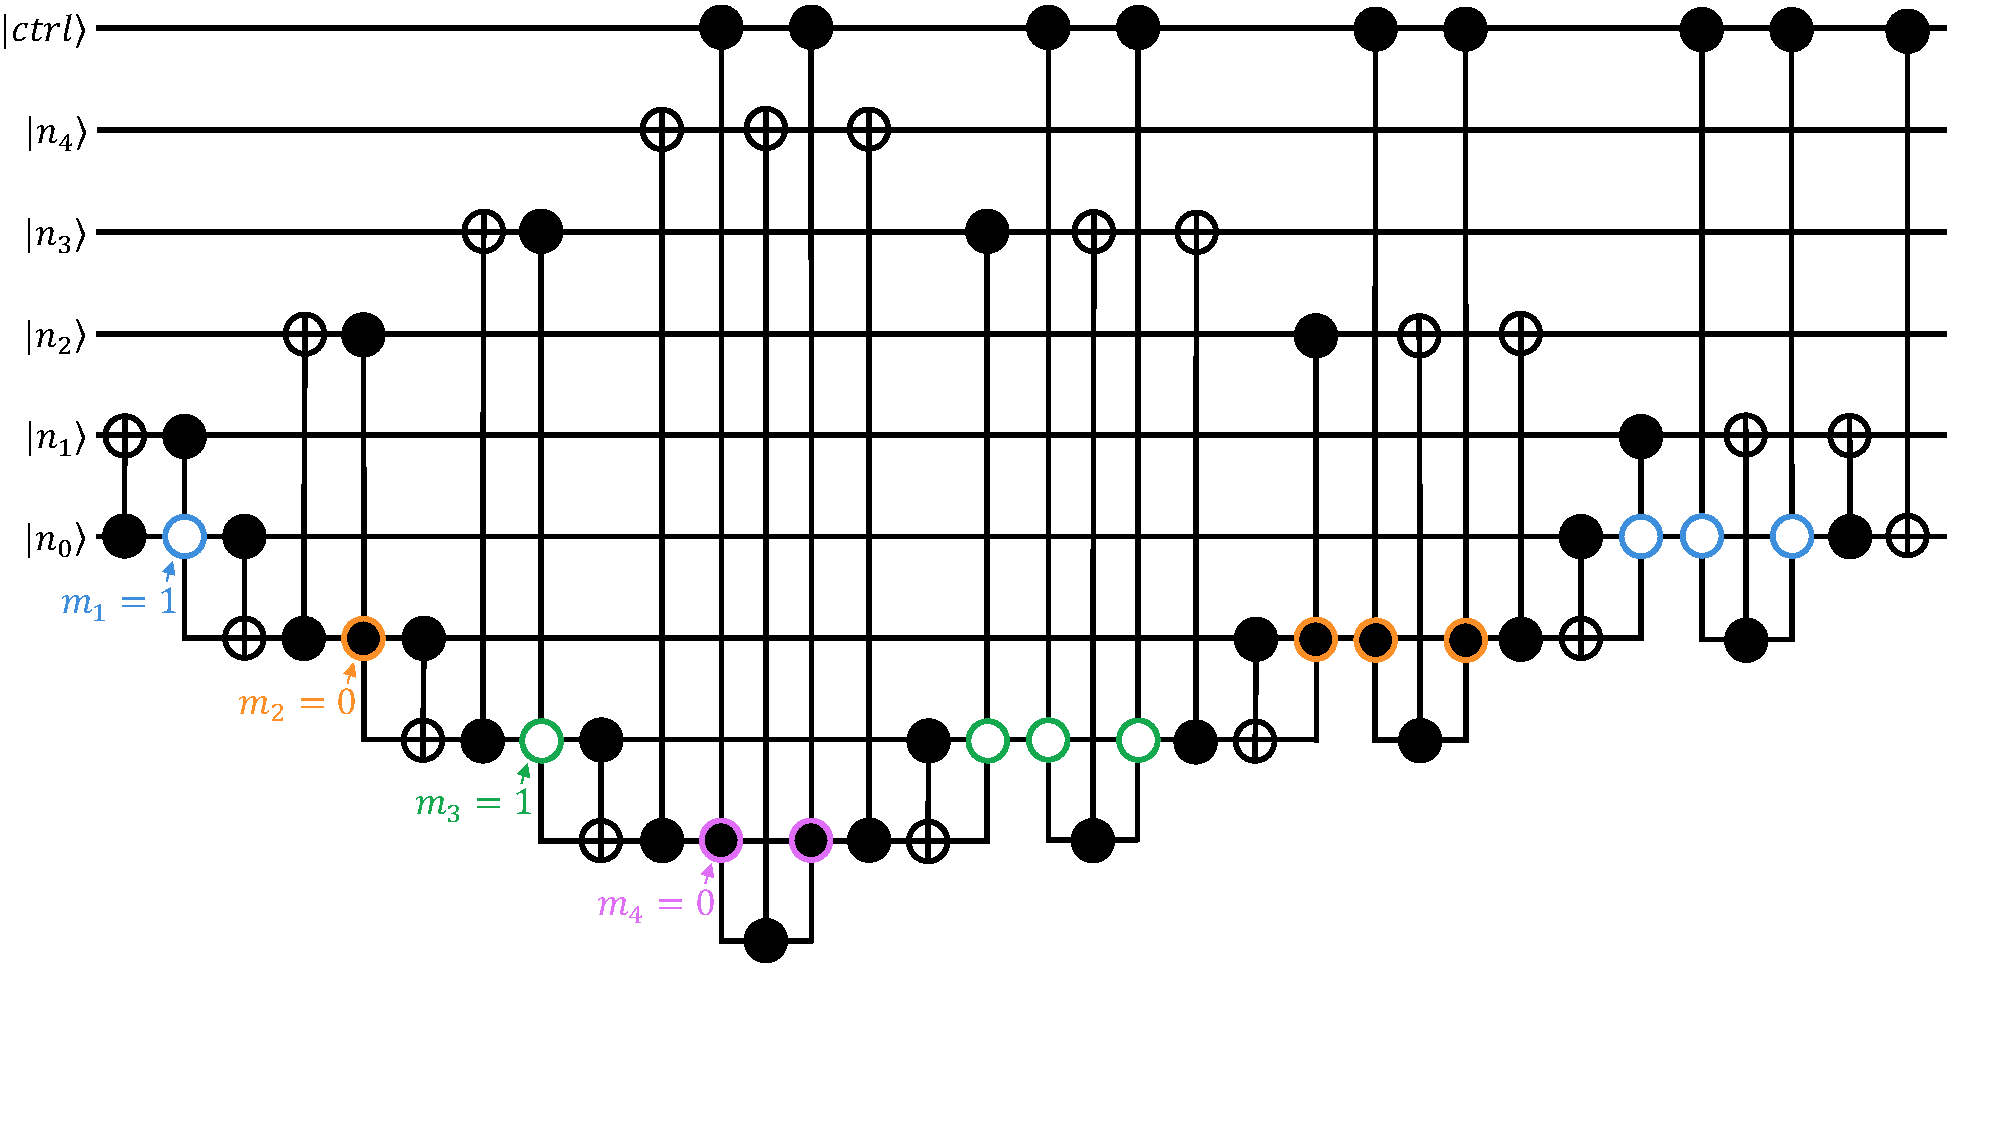
\includegraphics[width=12cm]{figures/ctrl-add-11-qubit-efficient.pdf}
    \caption{
        \textbf{Qubit-Efficient Controlled Addition of 11}
        The construction for controlled quantum addition given in \cite{gidney2018halving} can be modified to reduce the number of ancillae in the case that one of the values is a classical number.
        This diagram shows addition by the value $11$ which is given by $01011$ in binary with the left-most bit the most-significant.
        The values of the classical bits, $m_i$ where the $m_0$ is the least-significant bit, can be propagated into the control structure of the circuit.
        If the value of the bit $m_i$ is 0, the corresponding control in the circuit is controlled on the $\ket{1}$ state.
        If the value of the bit $m_i$ is 1, the corresponding control in the circuit is controlled on the $\ket{0}$ state.
        The value of the bit $m_0$ is assumed to be $1$ and is not depicted in the circuit.
        If the value of $m_0$ is $0$, the circuit can be bit-shifted as shown in Figure \ref{fig:addition-qubit-efficient-12}.
    }
    \label{fig:addition-qubit-efficient-11}
\end{figure}

\begin{figure}
    \centering
    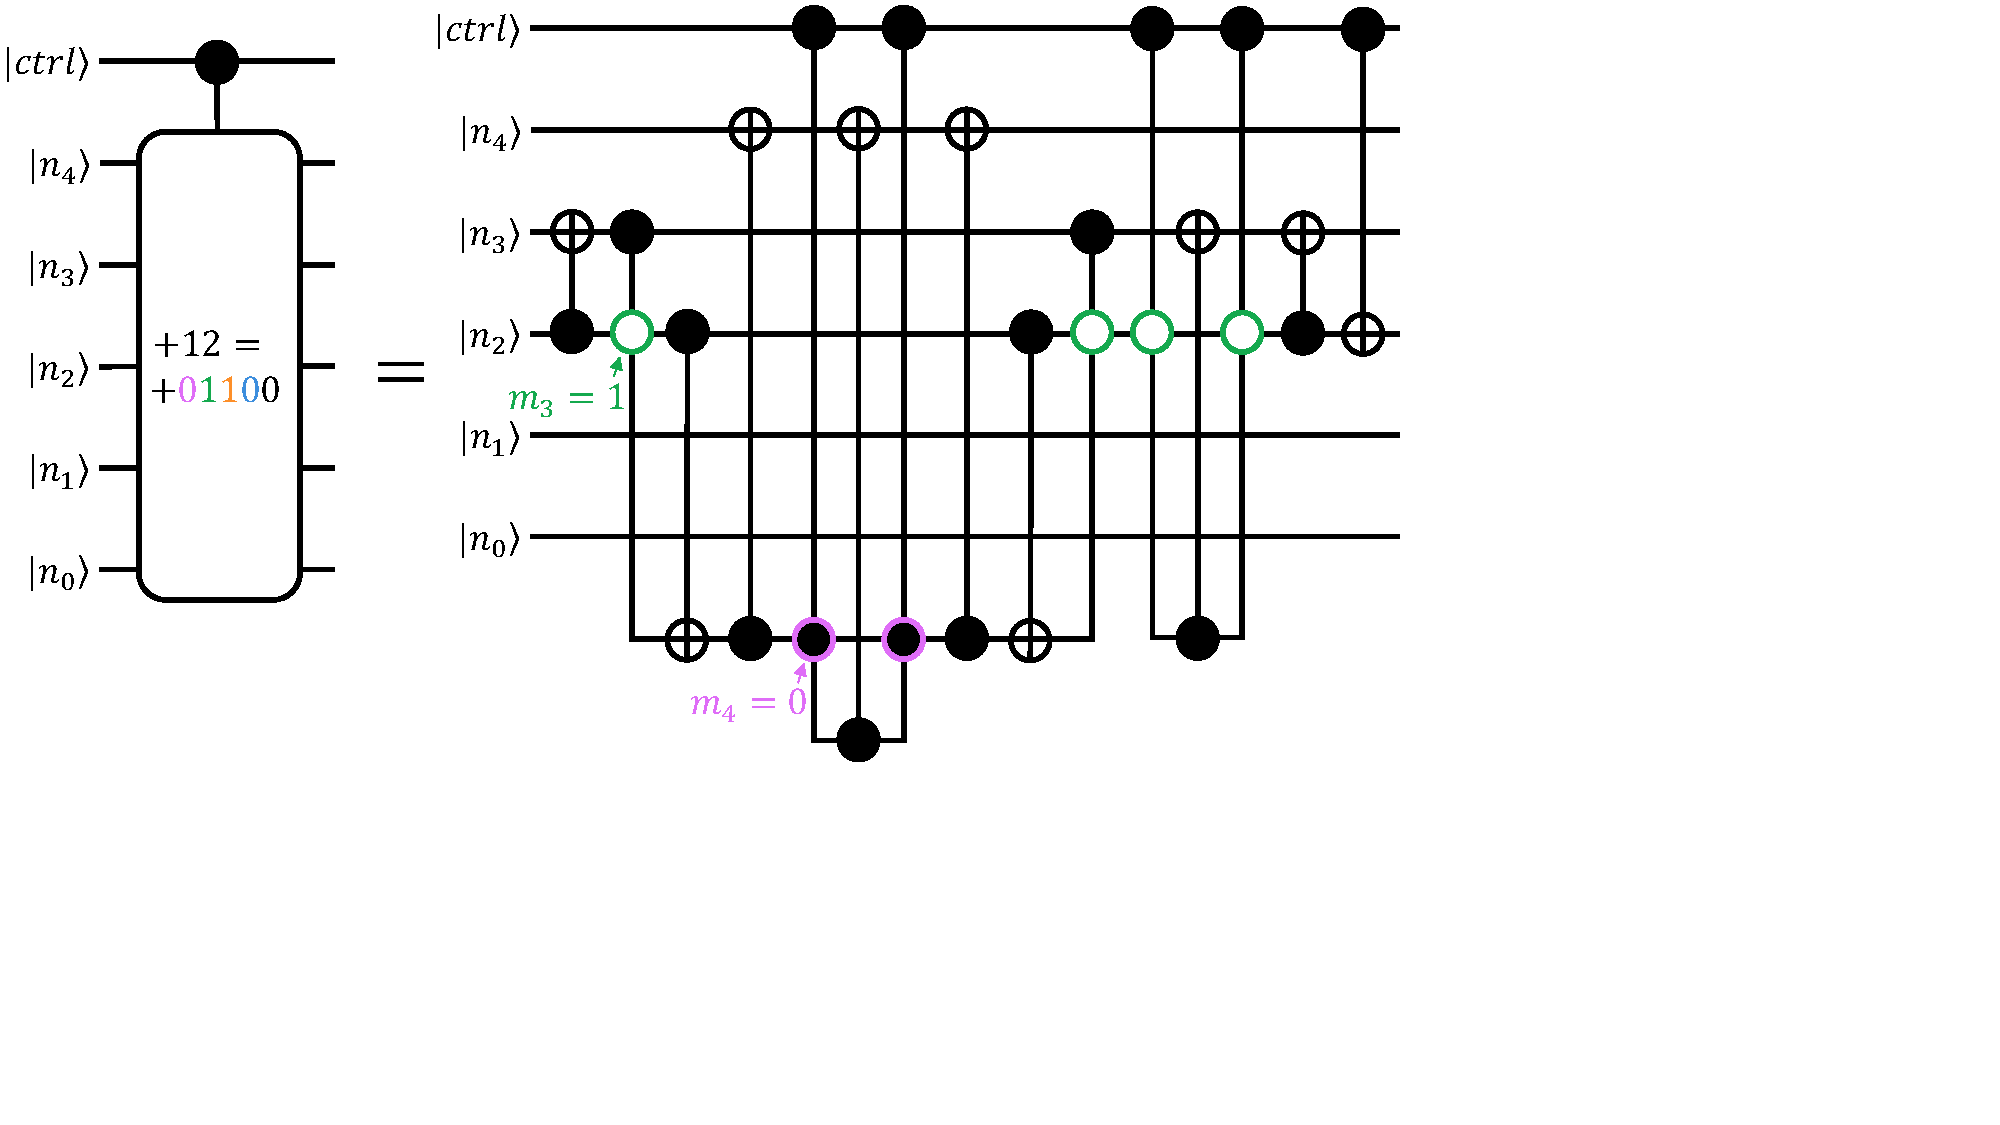
\includegraphics[width=8cm]{figures/ctrl-add-12-qubit-efficient.pdf}
    \caption{
        \textbf{Qubit-Efficient Controlled Addition of 12} 
        This circuit depicts the same protocol as in Figure \ref{fig:addition-qubit-efficient-11}, however, when the least-significant bit is $0$, the circuit can be bit-shifted to reduce the cost.
        This figure depicts the controlled addition of the value $12$ ($01100$ in binary).
        The two least-significant bits are $0$, so the circuit can be bit-shifted twice, significantly reducing the number of required operations.
    }
    \label{fig:addition-qubit-efficient-12}
\end{figure}

Another option is to use the same construction for the controlled quantum adder presented in \cite{gidney2018halving}, but to propagate the controls on the state of $\ket{m}$ into the circuit.
This method removes the register $\ket{m}$ from the quantum circuit, reducing the number of ancillae by $M$.
In Figure \ref{fig:addition-qubit-efficient-11}, we show a decomposition for this circuit when the number being added is $11$ ($01011$ in binary).
Additionally, since the lower bits of $m$ are known, the addition can be performed only beginning on the first non-zero bit of $m$.
An example of performing controlled addition of $12$ ($01100$ in binary) is shown in Figure \ref{fig:addition-qubit-efficient-12} where the $2$ least significant qubits are disregarded.
If the $p$ least significant bits of $m$ are zero, this reduces the cost to $2(N - p) - 3$ left (and right) elbows and $N - p - 1$ ancillae.

\begin{figure}
    \centering
    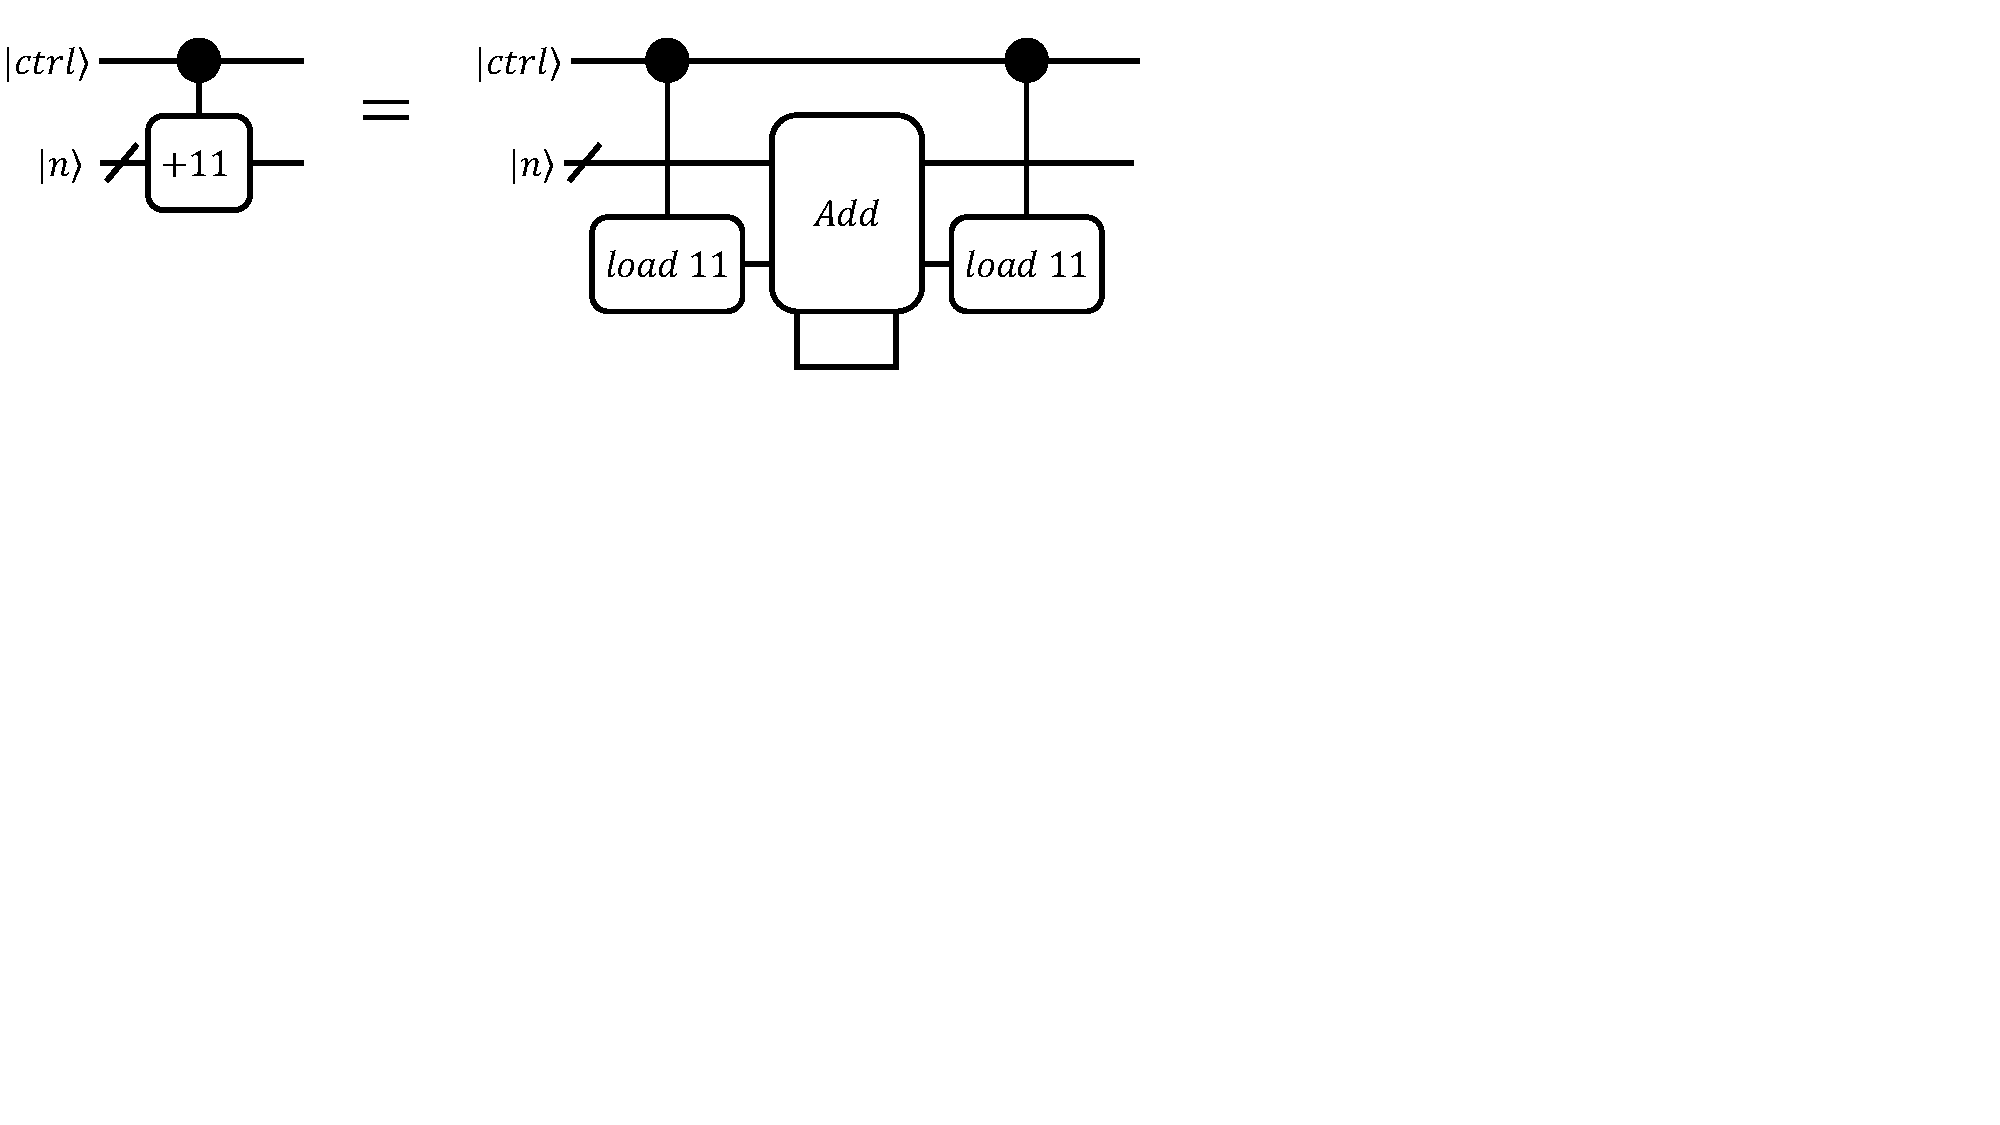
\includegraphics[width=12cm]{figures/ctrl-add-11-gate-efficient.pdf}
    \caption{
        \textbf{Gate-Efficient Controlled Addition of 11}
        The construction for controlled quantum addition given in \cite{gidney2018halving} can be modified to reduce the number of gates in the case that one of the values is a classical number.
        In this implementation, the classical value is loaded into an ancilla register which begins in the all-zero state (controlled on the control qubit) using a series of CNOT gates corresponding to the binary representation of the classical value.
        Next, the circuit for uncontrolled quantum addition given in \cite{gidney2018halving} is applied to the two registers.
        Lastly, the loading of the classical value is uncomputed.
        In the case that the control is off, the classical value is \textit{not} loaded into the ancilla register and the addition circuit performs addition of $0$.
    }
    \label{fig:addition-gate-efficient}
\end{figure}

Lastly, a similar trick using the classical information about $m$ to modify the circuit for controlled addition shown in \cite{gidney2018halving} can reduce the number of left (and right) elbows.
In this construction, the value of $m$ is first loaded into a clean register using a series of CNOTs that are controlled on the control qubit.
The CNOTs present are determine from the binary decomposition of $m$.
Then an uncontrolled addition between the registers $\ket{m}$ and $\ket{n}$ can be performed using the decomposition in \cite{gidney2018halving}.
Finally, the controlled loading of $m$ is then performed again to uncompute the ancillae qubits and return them to a useable state.
A diagram of this ciruit is shown in Figure \ref{fig:addition-gate-efficient}.
Overall, this requires $N - p - 1$ left (and right) elbows and $N + M - p - 1$ ancillae.
Since this option requires the fewest non-Clifford operations while only using a moderate amount of ancillae, this option will be used to determine the resource estimates used in this work.